\chapter{Photodetectors} \label{ch:photo_detectors}
As depicted in chapter \ref{ch:scintillators}, the detection of scintillation light is a crucial task when it comes to building detectors. Before semiconductor detectors like the \tit{photodiode} were invented, the \tit{photomultiplier tube} (PMT) was state-of-the-art for measuring up to single photons with low noise and high gain. Although PMTs are widely used, photodiodes provide attractive advantages in some cases. A short overview and comparison is given in this chapter. 
\section{Photomultiplier tube}
The photomultiplier tube is an evacuated glass tube with internal electronic structures. At the front, a photo cathode converts an incident photon from the light input window via the photoelectric effect into a photoelectron.  
\begin{figure}[b]
	\floatbox[{\capbeside\thisfloatsetup{capbesideposition={right,center},capbesidewidth=6.5cm}}]{figure}[\FBwidth]
	{\caption[Photomultiplier tube]{Cross section of a photomultiplier tube. The base for the PMT is mounted onto the pins on the bottom of the glass tube. Amended from \cite{wermes}.}   
	\label{fig:ch3:pmts}}
	{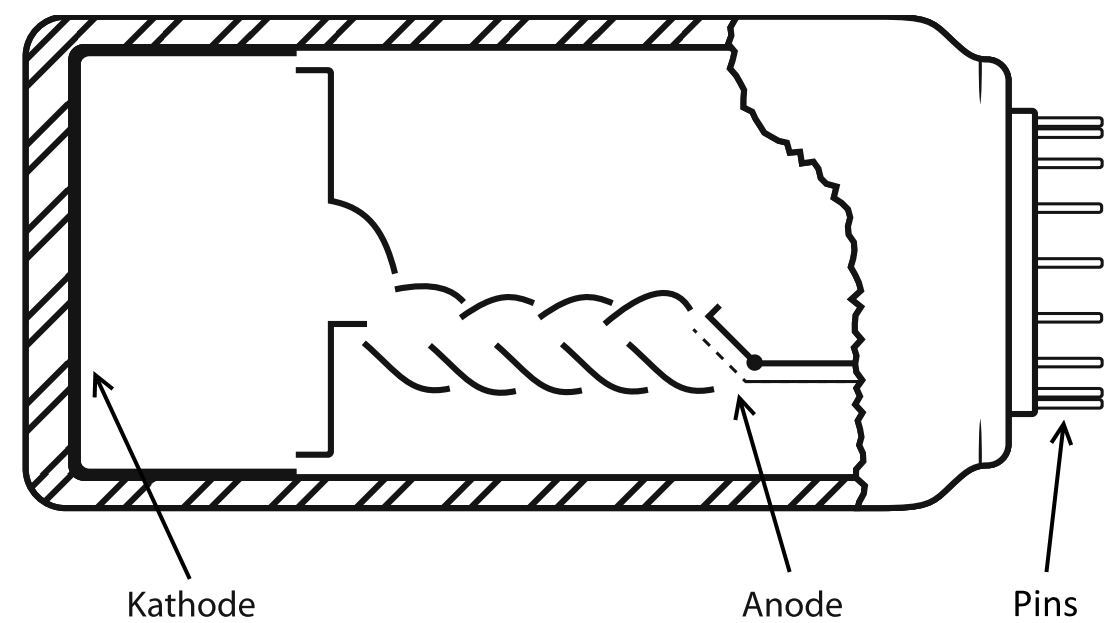
\includegraphics[width=0.5\textwidth]{./graphics/ch3/pmt1.png}}
\end{figure}
A strong electric field accelerates this electron, focused by a focusing element, towards a first electron multiplier (\tit{dynode}). The impact creates a cascade of secondary electrons which are then accelerated towards a sequence of dynodes. These structures can bee seen in figure \ref{fig:ch3:pmts}. After a \tit{transit time} of few tens of nanoseconds \cite{moore} the shower of electrons, now amplified by a factor of $10^{5}$ to $10^{9}$, reaches the anode where a measurable electric pulse is generated. \par 
A resistive voltage divider (\tit{dynode-chain} or simply \tit{base}) supplies the accelerating voltages for the dynodes and is attached to the pins on the bottom of the glass tube. In order to create sufficient acceleration, high-voltage (500$\si{\volt}$-2500$\si{\volt}$) is used. \par 
The \tit{quantum efficiency} (QE) describes the probability whether an incident photon is converted into a photoelectron or not. This ratio depends on the \tit{photocathode radiant sensitivity} (QS) which is defined as the quotient of incoming energy $N_{ph}\cdot h\nu$ and converted energy $N_{pe}\cdot e$:
\begin{align}
QS=\frac{N_{pe}\cdot e}{N_{ph}\cdot h\nu} \left[\si{\ampere\second\over\watt\second}\right].
\label{eq:quantum_efficieny_pmt}
\end{align} 
Typical quantum efficiency values vary between 25\% and 40\%. These values highly depend on the material used for the entrance window and the photocathode. Figure \ref{fig:ch3:pmt_sensitivity} illustrates the quantum efficiency for different wavelengths. For instance, measuring the fast scintillating component of BaF$_2$ necessitates the usage of a fused silica light input window with a bialkali photocathode. \par 
Albeit PMTs have a high gain, fast amplification, low noise and single photon sensitivity, they cannot be used in strong magnetic fields. Yet they can be operated in low fields by shielding with $\mu$-metal. In addition, PMTs rely on high operating voltages and are bulky to mount on scintillators. \par 
Considering these downsides, one has to use other photodetectors when it comes to strong magnetic fields, space constraints and low costs. These prerequisites can be found in medical applications (MRT) and high energy physics (large-scale detectors).
\begin{figure}[h!]
	\subfloat[Photocathode radiant sensitivity] {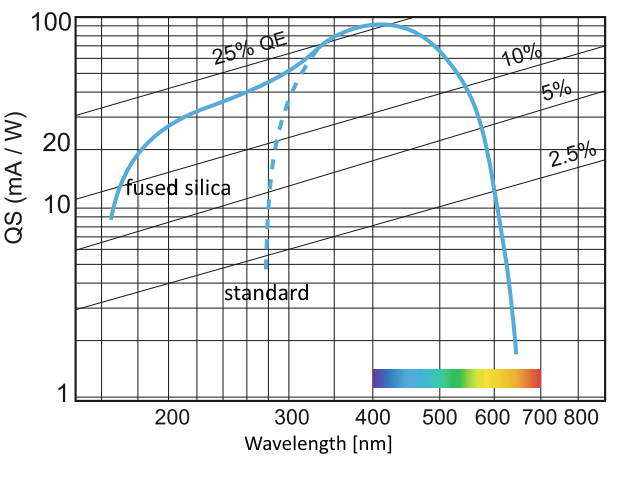
\includegraphics[width=0.49\textwidth]{./graphics/ch3/pmt_glass.png}}
	\hfill
	\subfloat[Photon emission spectra ] {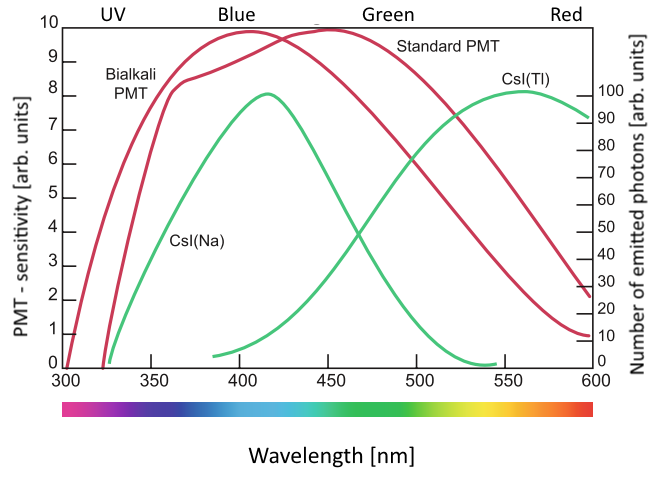
\includegraphics[width=0.49\textwidth]{./graphics/ch3/pmt_sensitivity.png}}
	\hfill
	\caption[Photon sensitivity of PMTs]{PMT wavelength dependency of photon sensitivity \cite{wermes}. The sensitivity for UV photons can be extended by using fused silica light input windows (a). To get the highest efficiency, the photocathode material has to be adapted for the emission spectrum of the scintillator (b).}
	\label{fig:ch3:pmt_sensitivity}
\end{figure} 
\section{Semiconductor detectors}
To solve some of the shortcomings of PMTs, solid state physics contributes a comprehensive class of materials, the semiconductors, which already have been introduced in chapter \ref{ch:semiconducters}. In the following, some applications will be presented.
\subsection{p-n junction}
The junction between a positive (p-) and negative (n-) doped semiconductor is called \tit{p-n junction}. In contact, free charge carriers (holes $h$ and electrons $e$) diffuse into the opposed region, leaving negative, respectively positive charged ions behind. Due to recombination, a \tit{depletion layer} between the p- and n-doped material is produced, which lacks free charge carriers. Since there are charged ions left, a \tit{built-in potential} forms and an electric field is generated (see figure \ref{fig:ch3:pn}). A stable condition attunes when the recombination stops and the drift and diffusion of holes and electrons compensate.   \par 
With \tit{reversed bias} (positive terminal attached to the cathode), the depletion layer broadens and the built-in potential intensifies. At a certain level of voltage $U_{BD}$, an avalanche occurs where electrons gain sufficient energy to create more charge carriers (\tit{breakdown}).  \tit{Forward biasing} (positive terminal attached to the anode) will shrink the layer and therefore lower the electrical resistance.   \par 
The p-n junction, as part of a circuit, is called \tit{diode}. 
\begin{figure}[h!]
	\floatbox[{\capbeside\thisfloatsetup{capbesideposition={right,center},capbesidewidth=6.75cm}}]{figure}[\FBwidth]
	{\caption[p-n junction]{Schematics of a p-n junction. It can be seen that the energy levels in the contact region are curved due to the different doping. The Fermi level adjusts to stay constant. The depletion layer inhibits positive and negative ions which produce an electric field. It is oriented from the n- to the p-junction. In equilibrium, the net currents of drifting and diffusing are equal.  Graphic amended from \cite{wermes}.}   
		\label{fig:ch3:pn}}
	{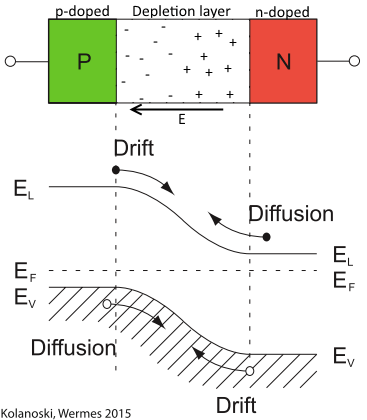
\includegraphics[width=0.5\textwidth]{./graphics/ch3/pn.png}}
\end{figure}

\subsection{Photodiode}

The design of a photodiode is based on the p-n junction structure with reverse biasing. Incident photons with sufficient energy excite an electron-hole pair in the depletion region, which is then separated due to the electrical field. Both charge carriers get accelerated towards their respective electrode and an electric pulse can be measured because of induction. \par 
A so called \tit{p-i-n} diode is shown in figure \ref{fig:ch3:diode}. An intrinsic sheet is placed between p- and n-doped layers. By applying reverse bias, a depletion region forms across the whole intrinsic sheet which then provides electron-hole pairs by photoexcitation. \par 
Made of silicon, a photodiode has a higher quantum efficiency and sensitivity on a wider wavelength spectrum compared to PMTs, although they have no intrinsic amplification, a smaller sensitive surface and rely on preamplifiers. To overcome some of these downsides, the \tit{Avalanche Photo Diode} (APD) was developed. \par
\begin{figure}[b]
	\floatbox[{\capbeside\thisfloatsetup{capbesideposition={left,center},capbesidewidth=0.35\linewidth}}]{figure}[\FBwidth]
	{\caption[Photodiode]{Cross section of a photo diode. For reverse biasing, the cathode is connected to the positive terminal. Amended from \cite{wermes}.}   
		\label{fig:ch3:diode}}
	{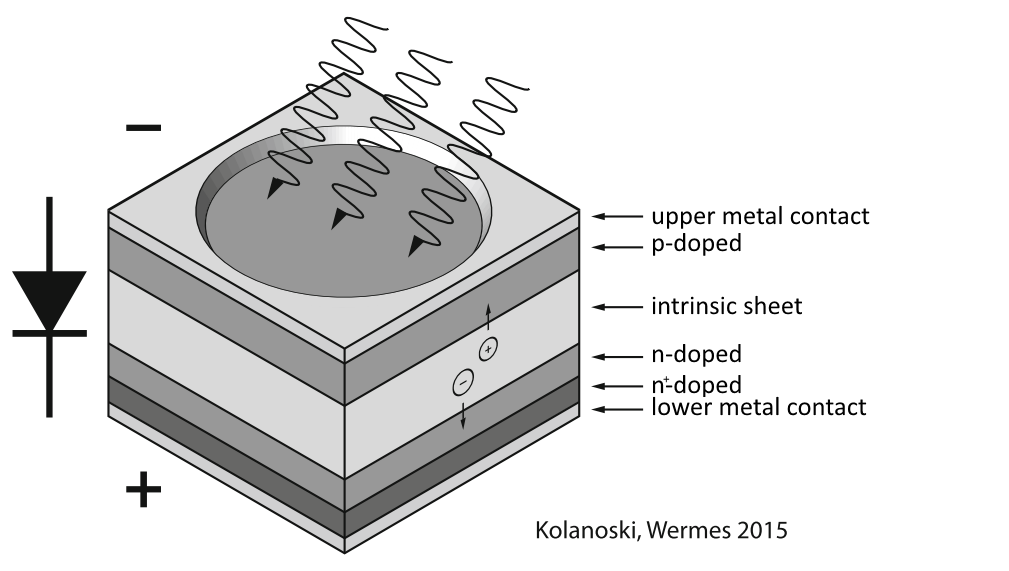
\includegraphics[width=0.65\textwidth]{./graphics/ch3/diode.png}}
\end{figure}
In addition to a single p-n junction, the APD integrates a second \tit{metallurgical junction} (highly doped p-n barrier junction) within the metal contacts. Incident photons excite h-e pairs in a thick, less-doped depletion region. The produced electrons drift through the depletion layer towards the readout electrode and pass the metallurgical junction. Since this barrier has a high electric field (up to $\SI{1}{\keV/\milli\meter}$ \cite{wermes}), the passing electrons gain energy and create secondary charge carriers through impact ionization processes. This avalanche continues and amplifies the signal up to a factor of \ten{2} to \ten{3}. \par 
To gain even higher amplification (up to \ten{5}), \tit{single photon APDs} (SPADs) can be operated in \tit{Geiger-Mode} where the supplied voltage $U_{OP}$ is set to 10\%-20\% beyond breakdown voltage $U_{BD}$. A single photon can trigger a self-perpetuating ionization cascade, the \tit{Geiger discharge}. To avoid any damage and to reset the APD, a series \tit{quenching resistor} $R_Q$ is used.  

\subsection{Silicon photomultiplier}

The \tit{Silicon Photomultiplier} (SiPM) integrates a large number of microcells ($\text{SPAD}+R_Q$) as an array in a dense area on a silicon substrate \cite{sensL}. The SPAD pixel size ranges from $\SI{15}{\micro\meter}$ to $\SI{70}{\micro\meter}$ \cite{buzhan}. Each pixel works binary, therefore the number of incident photons can be estimated by the number of pixels hit. The probability of multiple hits of a single cell is low since the packing density is high and the dead time is small ($<\SI{100}{\nano\second}$ \cite{wermes}). \par 
\begin{figure}[b!]
	\subfloat[N-on-P structure.] {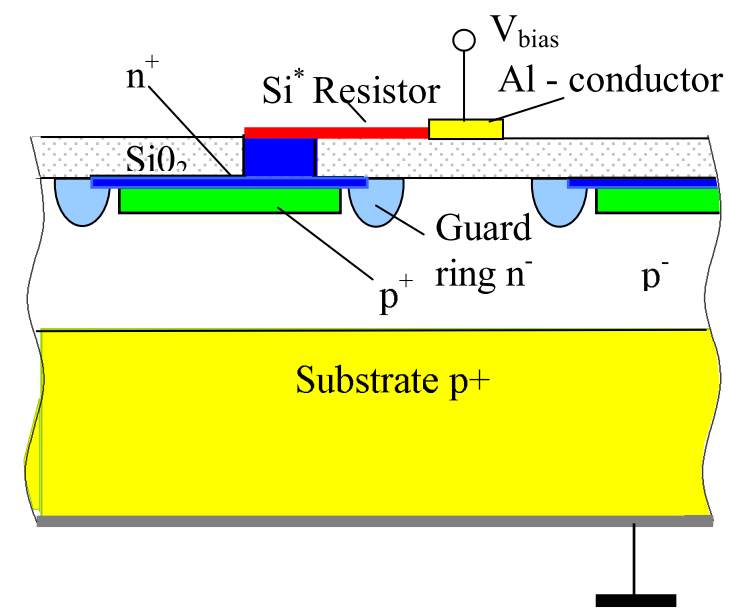
\includegraphics[width=0.45\textwidth]{./graphics/ch3/sipm_scheme.png}}
	\hfill
	\subfloat[\tit{KETEK} \tit{P-on-N} structure] {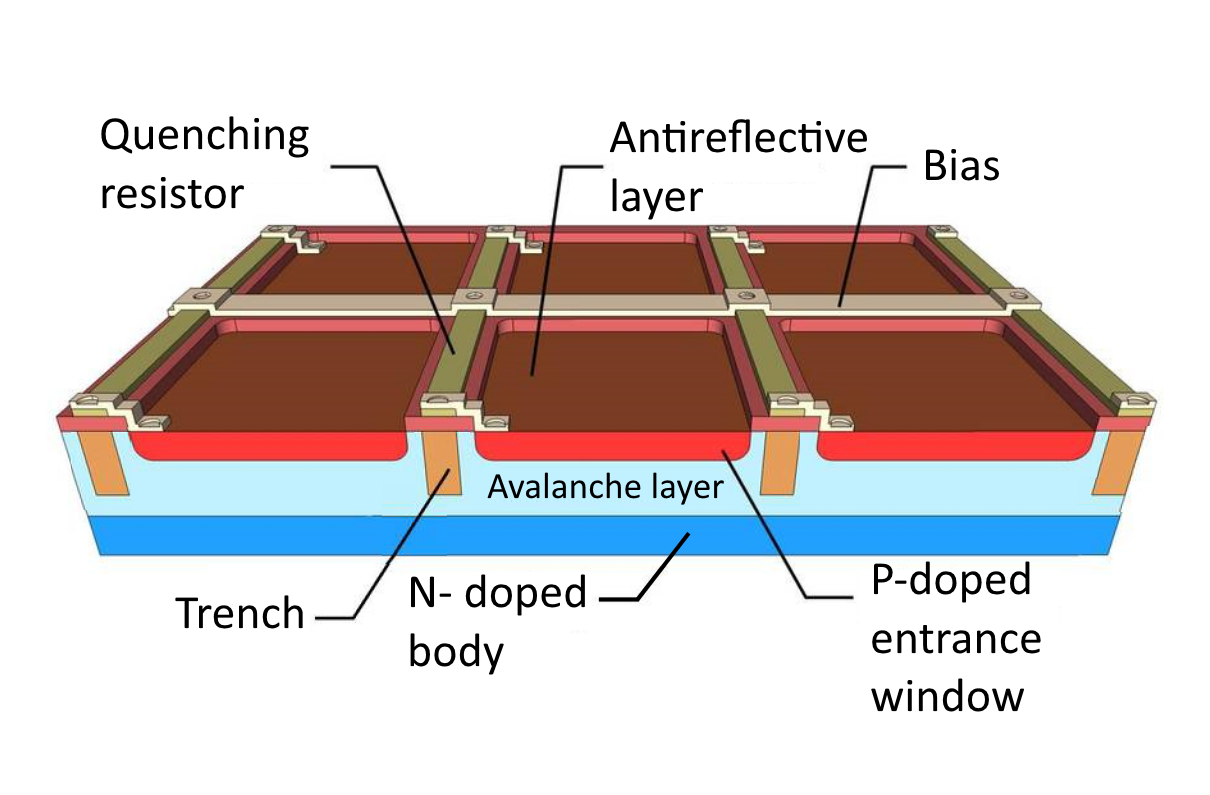
\includegraphics[width=0.54\textwidth]{./graphics/ch3/ketek_sipm_scheme.png}}
	\hfill
	\caption[SiPM schematics]{Different schematics of SiPM designs. N-on-P technology with guard-rings (a). P-on-N technology with trenches to avoid cross-talk by \tit{KETEK} (b). Amended from \cite{buzhan} and \cite{ketek}. }
	\label{fig:ch3:sipm_scheme}
\end{figure}
In figure \ref{fig:ch3:sipm_scheme} some SiPM schematics are shown. Incident photons are absorbed in the depletion layer (blue photons within $\SI{0.6}{\micro\meter}$, red photons within $\SI{2.9}{\micro\meter}$ \cite{wermes}) and the excited electrons drift towards the avalanche layer, where the amplification with a factor of up to \ten{6} happens and a signal is induced. The use of \tit{guard rings} avoids occurrence of surface currents and trenches avert, in combination with anitreflective layers, \tit{optical cross-talk} (photons emitted by avalanches escaping into an adjacent cell) to reduce noise. \par 
Since SiPMs work with low voltage ($<\SI{80}{\volt}$) and 10\%-20\% over-voltage, an avalanche has to be quenched with a resistor. When current is drawn by this resistor, the voltage drops below the breakdown voltage, the avalanche stops and the cell recharges. This generates a pulse with a short rise time of $\approx\SI{0.5}{\nano\second}$ and a tail with few hundreds of nanoseconds. \par 
Some further characteristics are the \tit{fill factor} (percentage of surface sensitive to light), the \tit{photon detection efficiency} (PDE, sensitivity as function of wavelength), the \tit{dark count rate} (count rate without exposure to light), \tit{afterpulsing} (delayed release of trapped carriers after primary breakdown) and temperature dependencies.




